\section{Implementation}

\subsection{Key Exchange}
While cryptography is an ever evolving field that seeks a balance between cryptographic integrity and system efficiency, the core of modern cryptography utilizes highly difficult or resource intensive mathematical problems. Historically, the backbone of public-key systems relies on the difficulty of prime factorization; there is simply no efficient algorithm to compute the factors of large numbers containing large prime numbers (though, this may change in the future with advances in mathematics or quantum computing). That is, it is quite easy to multiply two large numbers but very difficult to factor one large number. Thus, the difficulty of breaking such a cryptographic scheme correlates to the size of these numbers.

In 1978, Ronald Rivest, Adi Shamir, and Leonard Adleman developed the first public-key based encryption algorithm known as RSA. The security of RSA relies on the Discrete Log Problem (DLP). The discrete logarithm problem is defined as given a group G, a generator g of the group and an element h of G, find the discrete logarithm to the base g of h in the group G. The problem's difficulty depends on the group used, therefore certain groups are preferred when used for cryptography. For example, RSA utilizes the group of integers modulo a large number (~100 digits long) n, under integer multiplication. 

However, in 1985 two mathematicians independently proposed the use of elliptic curves in cryptography (ECC). An elliptic curve $E_k$ is defined over a field K such that its characteristic doesn't equal 2 or 3. For $a,b \in K$, an elliptic curve is the solution set of $(x,y)$ pairs in $K^2$ that satisfy the following equation: $y^2 = x^3 + ax + b$. After much mathematical research, points on elliptic curves can surprisingly comprise a group, and therefore, ECC can utilize the DLP similar to RSA, only with a different group. Namely, one can create an addition group law under the integer points of an elliptic curve. With this group in mind, one can integrate elliptic curves into other cryptographic schemes that utilize other forms of the DLP (e.g. Diffie-Hellman key exchange or digital signatures).

 %Example of addition group law on integer solutions on an elliptic curve
 \begin{figure}[t]
	\centering
	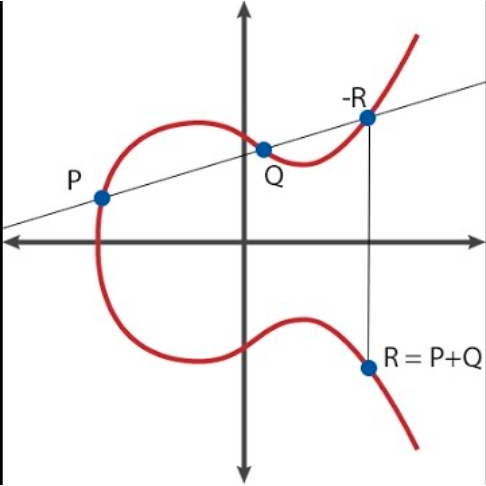
\includegraphics[width=5cm,height=0.5\textheight,keepaspectratio]{./figures/figure_1}
	\caption[font=footnote]{Example of addition group law on integer solutions on an elliptic curve}
	%\center{\footnotesize{Phase I}}
\end{figure}

ECC has a variety of applications in cryptography including elliptic curve Diffie-Hellman, digital signatures, and encryption. The preeminent advantage to using ECC is the ratio of key size to security strength. In Table 1 we can see a comparison of security strength and key size between symmetric keys, ECC keys,  and standard public-key schemes like RSA. The size of keys grows dramatically for equivalent strength in standard RSA keys while ECC key strength to key size ratio grows slowly. While ECC doesn't have the same strength to size ratio as typical symmetric cryptography this is a remarkable improvement over previous public-key crypto-systems such as RSA.

%From The Advantages of Elliptic Curve Cryptography in for Wireless Security by Kristin Lauter
 \begin{table}[t]
	\centering
	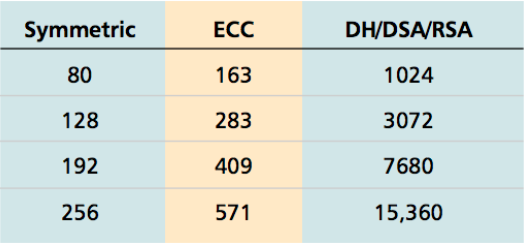
\includegraphics[width=9cm,height=0.5\textheight,keepaspectratio]{./figures/table_1}
	\center\caption[font=footnote]{Key Sizes for equivalent Security Levels}
	%\center{\footnotesize{From \textit{The Advantages of Elliptic Curve Cryptography in for Wireless Security} by Kristin Lauter}}
\end{table}
	
A study at Sun Microsystems Laboratory found that ECC-160 point multiplication outperforms the RSA-1024 private-key operation by an order of magnitude and is within a factor of 2 of the RSA-1024 public-key operation. This key size to strength ratio is beneficial to environments that have limited resource, such as IoT environments, since smaller keys allows for less memory usage, less data to transmit, and faster operations. There are a variety of curves to choose from when running or implementing ECC. The particular curve and naming convention denotes the size of the field over which the curve is defined. The curve name corresponds to the size of the key pair as well as the secret generated (through a Diffie-Hellman key exchange). Table 2 indicates a number of approved named curves as well as their properties and strength compared to size and standard RSA/DSA keys.

 
%Table 2 Curve properties 
 \begin{table}[t]
	\centering
	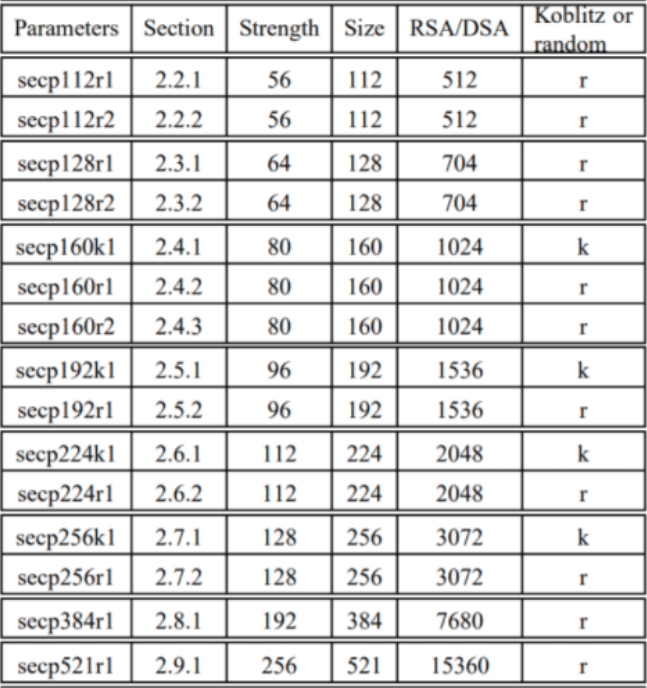
\includegraphics[width=9cm,height=0.7\textheight,keepaspectratio]{./figures/table_2}
	\center\caption[font=footnote]{Curve Properties}
\end{table}

All ECC functionalities in this project were implemented using open source code created by Bouncy Castle. As previously mentioned, Bouncy Castle has a distribution for the Java ME platform and proved to be a good candidate for implementation since the Bouncy Castle distribution provided much of the functionality (particularly in the way of ECC) that was heavily lacking the standard Java ME security library. As discussed earlier, choosing the right elliptic curve is important. In this project the default chosen was secp128r1. Smaller keys are better in restricted environments but there must also not be a major loss to security. Table 3 indicates the achievability of certain government standards by each curve. A $c$ indicates the curve complies with the standard, while an $r$ indicates it is explicitly recommended.

%Table 3 Curves recommended by trusted standards.5
 \begin{table}[t]
	\centering
	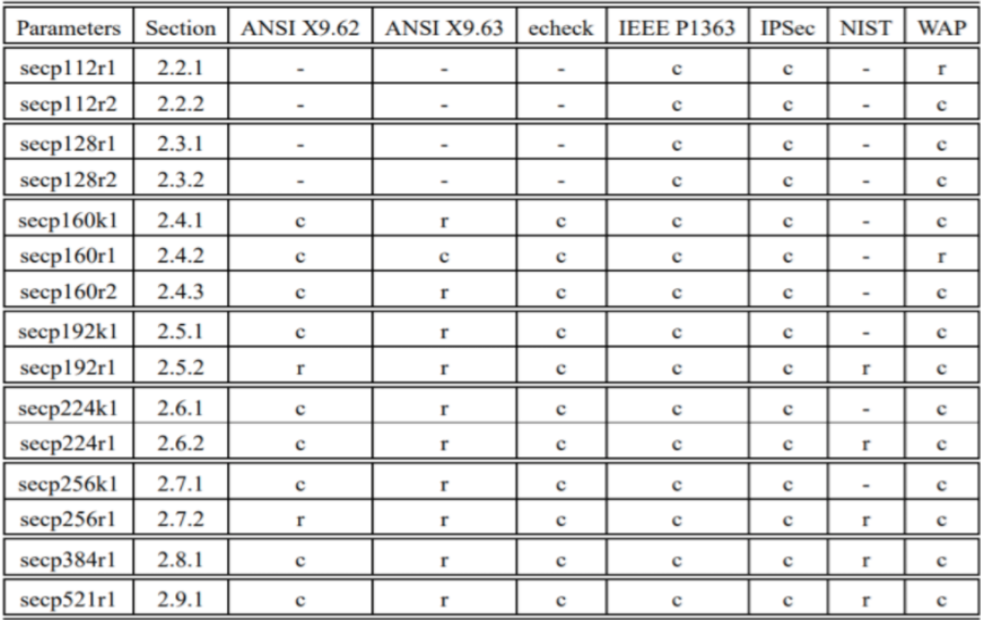
\includegraphics[width=12cm,height=0.7\textheight,keepaspectratio]{./figures/table_3}
	\center\caption[font=footnote]{Curves recommended by Trusted Standards}
\end{table}

While the secp128r1 curve is not always recommended, it does comply with several standards, and furthermore, keys generated with this curve produce a 128 bit key when used with ECDH for use as a symmetric key. It is recommended that symmetric key sizes do not fall below 80 bits, but 128 bit symmetric keys provide more security while remaining relatively small. Additionally, 128 bit keys allow us to use AES-128 rather than an encryption algorithm like TDEA. Although, in some circumstances it is viable to use secp128r1, it may be wise to use a curve with a larger field such as secp160r1 to generate the initial EC key-pair, then simply use the secret generated via ECDH to derive a smaller key (128 bits). Using a curve such as secp160r1 provides larger key-pairs, and in turn more security, which may be more beneficial for other forms of ECC, like the Elliptic Curve Digital Signature Algorithm (ECDSA). However, since the main goal of our implementation is to exchange a symmetric key to be used for encryption and authentication, it is more vital to focus on the strengths of this key. Therefore, as mentioned, the secp128r1 curve was used because it was the simplest way to produce a 128 bit secret. 

Functionality related to key generation, key pair generation, and key derivation, is provided in our KeyGen class. The implementation for EC key-pair generation in this project is straight-forward to use. Most parameters are taken care of without the need for users input, especially if the user simply uses the default parameters (i.e. secp128r1 curve, 128 bit key). There is room for users to choose a different curve and key size if desired. Bouncy Castle's implementation of ECC offers a number of different curves to be used, including all those in Table 2 and 3, as well as others not mentioned in the recommended curve list. It should be noted that the key size in this library refers to the secret size generated from the ECDH exchange. If a curve other than secp128r1 is being used the user must input the secret size(in bytes, not bits) that corresponds to the selected curve, otherwise an error will be thrown when attempting to generate a secret. If a distinct curve is desired, the proper secret size can be calculated by converting the field size to bytes. For example, the secp160r1 curve would generate a 20 byte secret, but if a smaller symmetric key is desired, it is possible to take this 20 byte secret generated and derive a smaller key using the key derivation function available in the class.

Key exchange was implemented using a version of Diffie-Hellman using ECC in the form of ECDH. The Diffie-Hellman key exchange protocol is popular in most crypto-systems. It's a rather clever protocol in which each party chooses a private key, say $G$ or $K$, calculates the corresponding public key $G_x$  or $K_y$ , and sends this public key to the other party. Once received each party can then calculate a secret number by combining the other party's public key with their own private key such as $(Gx)y$ or (Ky)x. This provides both parties with a secret key shared between the two that, while revealing the public keys, keeps the private keys secret, rendering the shared secret difficult to compute by malicious parties listening in. This is described by in Figure 2. 

Due to the nature of the algorithm, it can be easily converted to use ECC, as mentioned previously. In this project, Diffie-Hellman key exchange was implemented using ECC with Bouncy Castles open source deployment. The ECDH  implemented in this project is easy to use, straightforward, and can be used in conjunction with the key generation functionality. Users simply need to provide two AsymmetricKeyParameters (a class provided by Bouncy Castle). The parameters provided should correspond to the server's private key and the client's public key (as is typical in a Diffie-Hellman exchange). If the user has their key in bytes, functionality is provided to convert a byte array into the proper parameter. Executing ECDH will return a shared secret to the user in the form of a byte array.

 \begin{figure}[t]
	\centering
	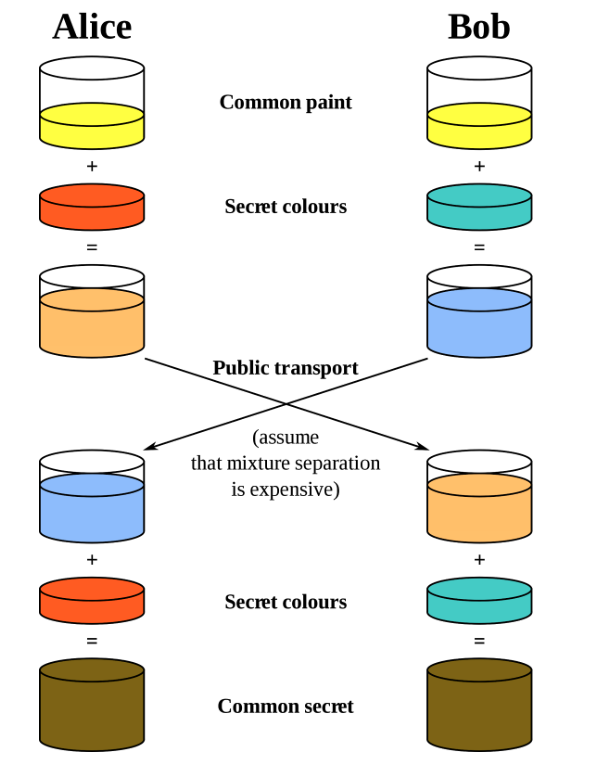
\includegraphics[width=9cm,height=0.7\textheight,keepaspectratio]{./figures/figure_3}
	\center\caption[font=footnote]{Diffie-Hellman Key Exchange}
\end{figure}

It's natural to touch on ephemeral versus static key pairs as this has an effect on performance and security. An ephemeral key pair is generated for one time use. The key pair will only be used during one connection and discarded afterward, this means that the identity of the sender is not necessarily verified and should be verified in another way. Static key pairs are kept for a longer period of time and can be used to verify the identity of the sender. In this library using ephemeral or static key pairs is left to the user, although, the functionality directly provides the ability for a ephemeral scheme and therefore using a static scheme requires extra help for initial authentication (this can be accomplished with a certificate chain but this is not in the scope of this project). Ephemeral keys offer the benefit of forward security, which is the idea that (since keys are only used once per connection) sensitive data from previous connections cannot be compromised. However, using ephemeral keys has its drawbacks as well, including more overhead from key generation, and the lack of authentication. Since the ephemeral keys are only used once, they must be accompanied by another form of authentication during the initial connection. In this project, this is left up to the user. Static keys on the other hand allow malicious persons to compromise all past data that was passed using that given key pair. Though this lowers the security of the scheme, it also means that the same key is used multiple times which relieves some overhead from key generation, as well as providing the authentication needed at the initial connection. Either scheme has benefits and drawbacks but still perform the function of providing a shared secret between two parties.

\subsection{Encryption}

While it is possible to use a shared secret directly as a key, it is recommended to use this shared secret to derive a new key. However, this requires both parties to use the same key derivation formula. Key derivation is the act of taking a secret value, such as a password, shared secret, or passphrase and creating one or more secret keys. The act of deriving a key allows a party to take one key that may not meet proper format and converting it to the correct size. Most key derivations use hash functions to produce a given output size. Occasionally, they add additional non-secret parameters to add entropy to the derived key; this is known as key diversification. In this project, a simple key derivation formula was devised and is relatively easy to use. The MD5 hash algorithm is used by default due to its relative security and an output of 128 bits. This function takes both the parties public keys used in the exchange, and hashes them with the shared secret. It's important to note that the public keys should be updated at the same time for both parties. This means that parties on both sides of the communication must put the public keys in the hash algorithm in the same order. Failure to do this will result in a different derived key and any attempted secure communication will fail. Luckily, our function rearranges the public keys in the correct order for the users. The key derivation function will produce any size key as specified by the user. This means that a variable length secret can be converted into a specified length simply by specifying the desired length in the parameters and given the proper digest. 

Once a symmetric key has been exchanged and/or derived users may begin exchanging encrypted data. Perhaps the most common symmetric ciphers used for encryption and decryption in modern systems is AES, also known as the Advanced Encryption Standard. It was first published by Vincent Rijmen and Joan Daemen in 1998, and it superseded the Data Encryption Standard (DES).  Originally adopted by the U.S. government, AES is now widely spread as the standard cipher for symmetric encryption. In this project, it sufficed to simply use AES since our default key size matched the block size for AES at 128 bits. Additionally, Java ME's standard library also provides the ability to implement AES encryption. The implementation in this project provides users with a relatively simple interface for encrypting data with AES given plaintext and a symmetric key. Given a plaintext and key in the form of byte arrays, the function will automatically pad the plaintext to fit the proper multiples of the block size of 128 bits (16 bytes) when needed. Once padded, the plaintext is encrypted using the provided key and returns ciphertext in the form of a byte array. Similarly, the decryption function  takes ciphertext and the corresponding key and returns the plaintext. 

\subsection{Authentication and Integrity}

 \begin{figure}[t]
	\centering
	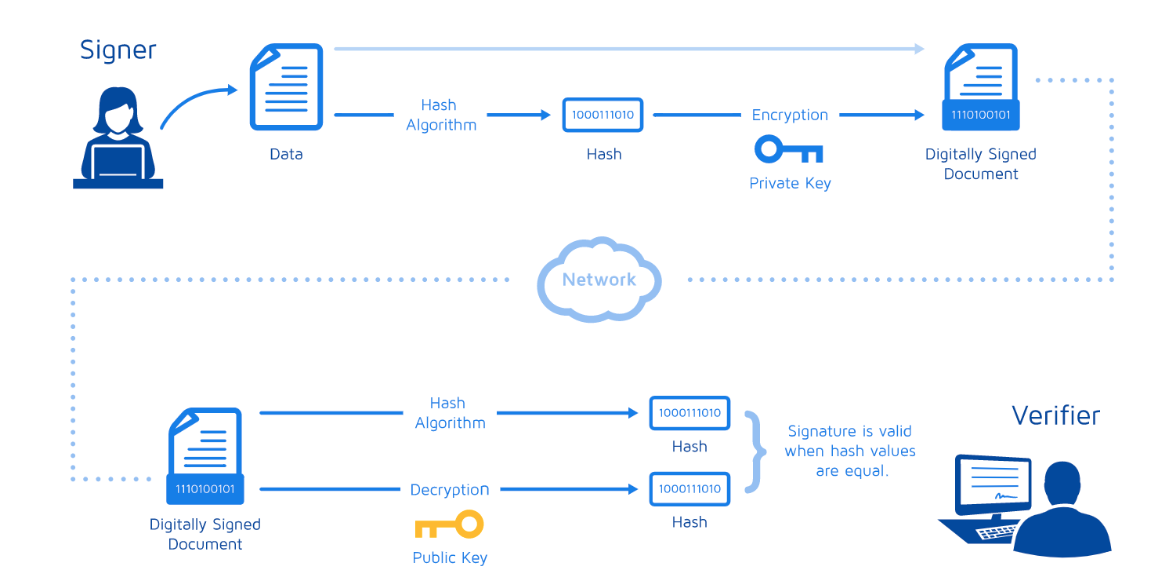
\includegraphics[width=14cm,height=0.7\textheight,keepaspectratio]{./figures/figure_4}
	\center\caption[font=footnote]{Digital Signature Process}
\end{figure}

Finally, our security library provides functionality for authentication and data integrity. Many systems provide authentication and integrity through the form of digital signatures using algorithms such as Digital Signature Algorithm (DSA) or its elliptic curve counterpart (ECDSA). Digital signatures use asymmetric key-pairs to "sign" messages and offer three applications: authentication, integrity, and nonrepudiation. To achieve authentication a private key is used by the sender to encrypt a given message, and receivers can use the sender's public key to verify this signature by decrypting the message. Typically, the message is first hashed to compress the data and add the ability to check data integrity. Once the message is hashed, it is then encrypted using the sender's private key.  The sender sends both the original data (possibly encrypted using a symmetric key), along with the signed hash. The receiver then decrypts the hashed message, and hashes the original message. If the hash sent by the sender and the hash computed by the receiver match, then the data has remained intact and has not be tampered with by malicious forces. Digital signatures also offer the benefit of non-repudiation. This is the idea that a sender cannot later deny sending any given message since, by design, the sender must use their private key. Additionally, those who have possession of the sender's public key cannot maliciously fake a digital signature from the sender.

Although digital signatures are a powerful scheme for providing authenticity and integrity, they also add quite a bit of overhead. As previously discussed, asymmetric encryption and decryption take an enormous amount of time and resources compared to symmetric cryptography. Fortunately, we can achieve much of the same functionality with symmetric cryptography in the form of a Message Authentication Code (MAC). MACs can provide authentication and integrity similar to digital signatures but do not provide non-repudiation. However, message authentication codes are based on symmetric cryptography rather than asymmetric cryptography and are therefore much faster. Most digital signatures are used prior to the establishment of a shared secret or when non repudiation is critical. In an IoT environment, speed and resource efficiency are critical, so it's natural to implement MACs over digital signatures, even given the lack of non-repudiation. 

 \begin{figure}[t]
	\centering
	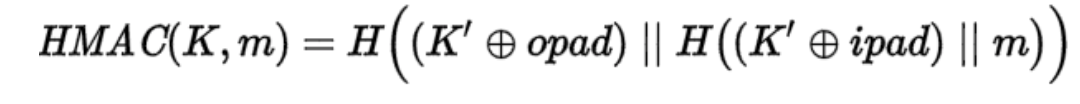
\includegraphics[width=9cm,height=0.7\textheight,keepaspectratio]{./figures/figure_5}
	\center\caption[font=footnote]{HMAC Algorithm}
\end{figure}

Message authentication codes offer authentication and integrity in much the same way as digital signatures but rather than using a key pair, they use a shared secret or symmetric key. Typically a message is generated and encrypted using AES, this encrypted message is then pushed through the given MAC function. There are a number of ways to implement MAC functions; typically implemented using hash based algorithms, known as HMACs, or cipher block algorithms, CMACs. Our security library implements the MAC in the form of a HMAC. While some hardware optimizations may make CMACs faster than HMACs, hashing algorithms typically add less overhead than cipher block algorithms. Therefore, HMACs are more suitable for an embedded environment. 

A user inputs a symmetric key and message into the HMAC, and the key is truncated or padded to the proper block size. This key is then XORed with the value $0x5c$. The non-XORed key is then also XORed with the value $0x36$, and the result is concatenated with the input  message. This concatenation is then hashed using the specified hash algorithm. The resulting hash is then concatenated with the initial XORed key value, and once again hashed using the specified algorithm. The final result produces the HMAC. To check the message's authenticity and integrity, the end user must recompute the HMAC using the shared symmetric key along with the received message. If the result is the same as the HMAC received, then the end user knows the message is valid.

It's important to note that the order in which a message is encrypted and the MAC is formed makes a difference in security. By encrypting a message and passing the cipher text into the MAC algorithm rather than passing the plaintext means that integrity is provided not only for the plaintext but also for the ciphertext. Additionally, if the encryption is malleable then the MAC will indicate any tampering with the ciphertext. If plaintext is passed rather than ciphertext, the MAC does not provide integrity for the ciphertext and it is theoretically possible to alter a message to appear valid when it is not if the given the cipher scheme is malleable. Though the implementation in this library does not explicitly execute this way, users who access the library should remember this fact when integrating these functions in their programs.

 \begin{figure}[t]
	\centering
	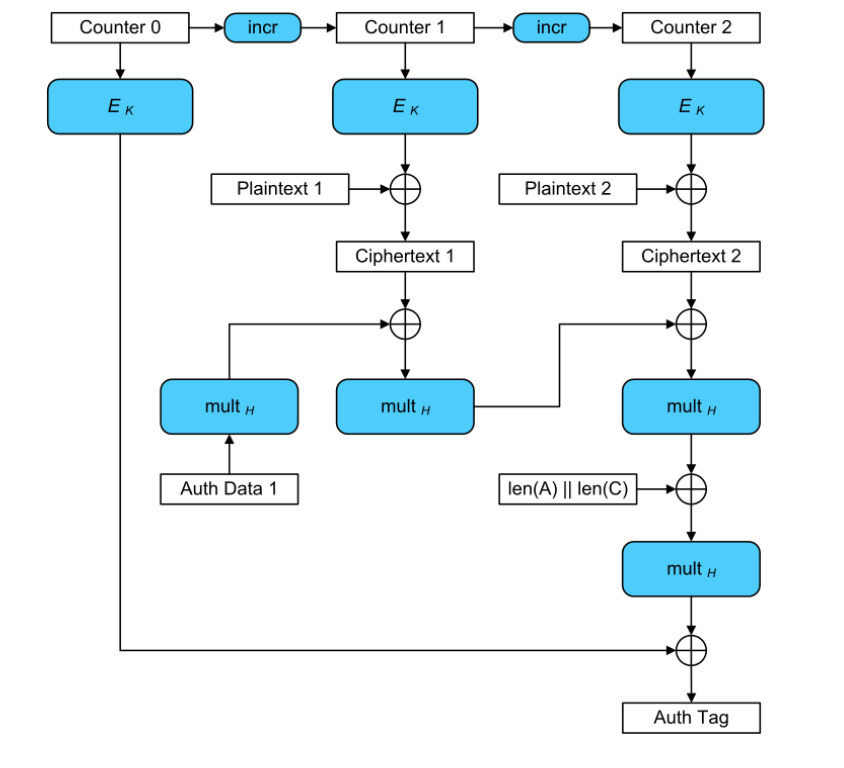
\includegraphics[width=12cm,height=0.7\textheight,keepaspectratio]{./figures/figure_6}
	\center\caption[font=footnote]{Galois Counter Mode Operations}
\end{figure}

Our implementation is relatively simple to use since only the key and data are required as input for authentication. Similar to most functionalities of this project, the HMAC uses the open source Bouncy Castle distribution. This data should be encrypted prior to being MACed. The  default hash function used is MD5 since its output is 128 bits and we wish to have smaller MACs while operating in embedded environments. While MD5 is the default, a different digest may be used at the user's discretion. All HMACs are returned as a byte array and can be easily verified by supplying the MAC, shared key, and original message. The verification function uses the HMAC function to recompute MAC and compare it to the received MAC. When they are the same, the function returns true, otherwise it returns false. 

Another methodology to provide authentication and integrity is to utilize the Galois Counter Mode (GCM) mode of operation for a symmetric block cipher. This mode of operation can be used in symmetric block ciphers to add authentication and integrity while it encrypts the data. This differs from simply using a MAC function because it is a mode of operation used in \textit{conjunction} with a cipher algorithm. The block size for GCM is 128 bits which is perfect for this library as it matches the default key size used. GCM requires users to supply: a secret key, a nonce, plaintext, and the additional data to be authenticated. The secret key is typically the symmetric shared secret or derived key between two parties. A nonce must be randomized for each message and is used as a counter. The nonce does not necessarily need to remain secret and can therefore be passed as plain text. However, it is crucial to make sure the nonce is not reused as this will depreciate the level of security. The plaintext required is simply any data that requires encryption, authentication, and integrity checks. Additional data is data that does not need to be encrypted but should be checked for authenticity and integrity. Running GCM will return both encrypted data along with an authentication tag (MAC). 

Galois counter mode works like many other counter modes associated with encryption. However, GCM provides a MAC as well. The operation of GCM is as follows. First a nonce is supplied in conjunction with a counter. This value is encrypted using the supplied key and XORed with the first block of the plaintext to produce a block ciphertext. This ciphertext will be used in our output but is also used to compute a MAC during operation. To compute the MAC, this block of ciphertext is multiplied with the key in what is known as a Galois field. The result is XORed with the next cipher block that is computed in the same way as the first. Often, the additional (non-encrypted) data is multiplied and XORed with the ciphertext before the next operation. This continues until all plaintext is encrypted and both ciphertext and a MAC are produced.  Decryption works similarly, the user must provide the ciphertext, secret key,  along with the authentication tag to decrypt and authenticate the data transmitted. Below is a diagram outlining the operation of GCM. 

In this project GCM was implemented using Bouncy Castle's open source distribution. The functionality implemented in this library allows users to provide a key, plaintext, nonce and associated data. Although a nonce is required, functionality for generating a nonce is provided in the class. The encryption function will return a single byte array containing ciphertext and the authentication tag. Decryption is simple to use as well, end users must provide the proper secret key, ciphertext, associated data, and nonce. If the MAC does not match the MAC provided, an error is thrown. The GCM encryption can be used in place of simply using AES and generating a separate MAC to provide integrity and authentication. 

\subsection{Results And Analysis}
We ran tests using the functions developed for our library on both an Intel Galileo Gen 2 and a Macbook pro to see the difference in runtime and determine if the speeds on the Galileo are feasible for real world applications. The results of our tests are as follows in Figure 7 and Figure 8 respectively.

%Galileo Gen 2
 \begin{figure}[t]
	\centering
	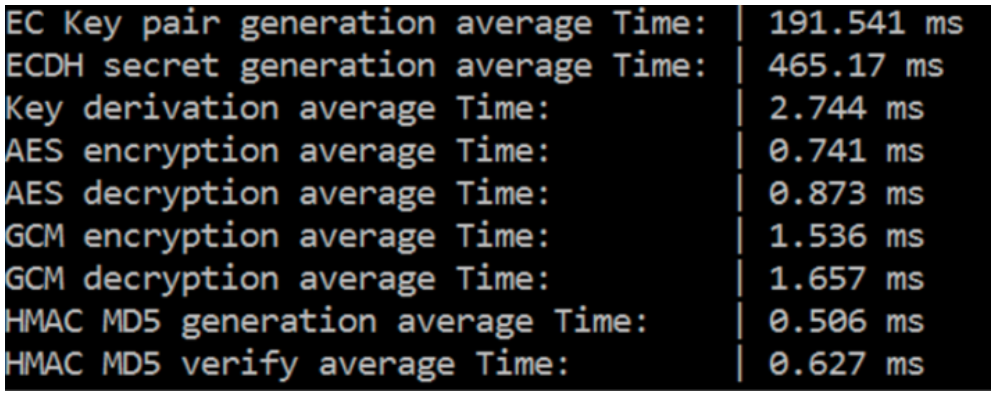
\includegraphics[width=12cm,height=0.7\textheight,keepaspectratio]{./figures/figure_7}
	\center\caption[font=footnote]{Average runtime for functions from our library run on the Galileo Gen 2}
\end{figure}

 \begin{figure}[t]
	\centering
	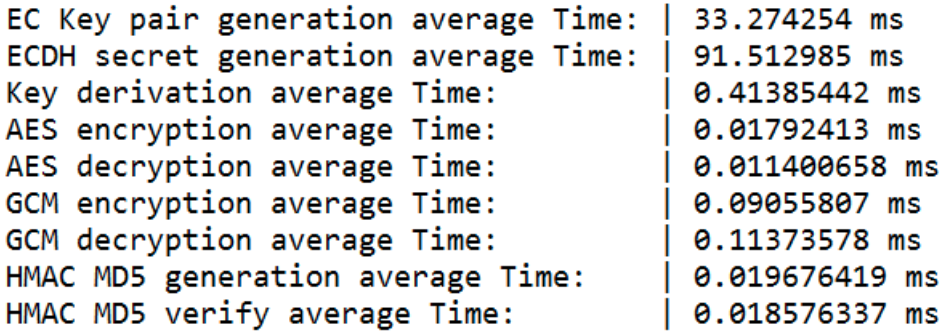
\includegraphics[width=12cm,height=0.7\textheight,keepaspectratio]{./figures/figure_8}
	\center\caption[font=footnote]{Average runtime for functions from our library run on the Macbook Pro}
\end{figure}

%Macbook

As expected the Galileo Gen 2 did not perform as well as the Macbook Pro. However, the numbers for the Galileo are not overly burdensome. The ECDH secret generation took the longest amount of time by far but was still a reasonable speed. If secrets are reused for a period of time the overhead of secret generation will be marginal. EC Key pair generation had the second longest runtime and surprisingly was less than the secret generation. Similar to the usage of a shared secret (symmetric key), prolonged usage of a key pair may help cut down overhead but depending on the application using ephemeral key pairs may be viable. Another surprising result is the runtime of AES in GCM mode versus the combination of AES and HMAC. Since GCM is renowned for its speed and efficiency it is surprising that the average run time of GCM is still greater than the runtime for both AES encryption and the generation of an HMAC combined.

To conclude, while run times on the Galileo were significantly worse than those on the Macbook, this was expected.  It was surprising to find that many of these algorithms ran at the speeds measured considering the Galileo's low resources. Although the Galileo is more powerful than many IoT devices, it is not unreasonable to assume Smart Home appliances could use this library as an addition to security.